\section{Introduction}
\label{section_intro}

\begin{figure}
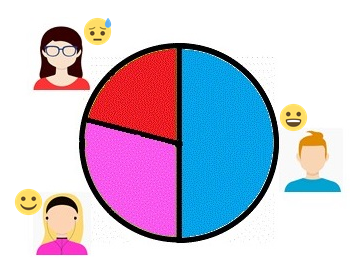
\includegraphics[width=2in]{images/cake_cutting.png}\Description{Cake-cutting Problem}
\caption{Fairness in cake cutting problem}
\end{figure}

Resource allocation has been one of the primary focus areas of economics since the beginning. It is also one of the most extensively studied one. The real-world is composed of limited resources as well as limited number of people who are going to use those resources. The problem of allocation of resources applies to both conditions in which, on one side, the resources are abundant (excess supply) or the other side where the number of users are larger (excess demand). Even with enough quantity of resources and consumers, each consumer may have different priority for different kinds of resources resulting in a complex allocation problem.

Two important concerns, among many others, in a resource allocation problem are efficiency and fairness. Efficiency criteria try to maximize the value that can be extracted from the available resources. Different types of efficiency criteria exist in resource allocation problem. One criterion may try to achieve the maximum possible value while other may try to optimize the utilization of all the available resources. We study some of these in greater details further in the paper. The fairness criterion tries to achieve overall welfare/goodness for all of the agents involved in the allocation problem. The idea of fairness have different perspectives depending upon the problem being studied. That may include equitability, where every agent gets an equal share in the allocation depending upon the agent's own subjective evaluation of the idea of equal share. Another interesting fairness perspective, which has gained much attention in the economics of fair allocation is envy-freeness. Envy-freeness ensures each agent prefers and values its own allocation more than the allocation of any other agent. We study this in more details in later sections.

The efficiency and fairness criteria are well studied for various types of goods in the market. One classification of such goods is based on divisibility. A divisible good, as the name suggests, can be described as the one which could be divided in fractions to achieve some form of allocation between multiple agents. Cake-cutting is a famous fair division problem with divisible goods. In cake-cutting problem, we need to divide a cake (or $m$ pieces of cakes) among some number of people in the party. \citet{varian1973equity} proposes competitive equilibrium for equal incomes (CEEI) for such a fair division problem. In CEEI, all agents are given equal income for fairness. Then each agent spends the income on some goods based on the agent's value for the good. In the cake division problem, a young individual may spend more to get a larger portion of the cake than an old person. The allocation is fair in terms of envy-freeness as each agent prefers its own allocation based on the value it has for that allocation. If it has more value, it will spend more to get larger fraction of the divisible good.

\begin{figure}
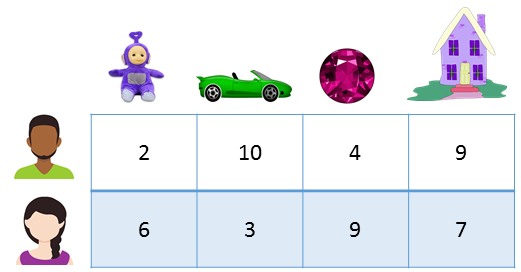
\includegraphics[width=3in]{images/indivisible_allocation2x4.png}\Description{Indivisible goods in Inheritance distribution}
\caption{Utilities of indivisible items in inheritance allocation}
\end{figure}

Introduction of indivisibility in goods takes away the envy-free property of the CEEI. More generally, envy-free solution does not exist for indivisible goods. Consider a simple resource allocation problem with one good and two agents. Since the good is indivisible, only one agent may get the object. The other agent will always envy for not getting the good. \citet{budish2011combinatorial} defines an approximation of the envy-freeness property for approximate-CEEI with indivisible goods. \citet{budish2011combinatorial} defines envy-freeness up to one good (EF1) as an approximation for envy-freeness and proves CEEI to be EF1 for additive utilities.

A welfare criteria we analyze in this paper is Nash social welfare. Nash social welfare is the product of values of allocations for each agent. An allocation which maximizes the Nash social welfare has interesting efficiency and fairness properties. The allocation problem solved by maximum Nash welfare (MNW) is envy-free for divisible goods. \citet{caragiannis2016unreasonable} shows MNW to provide efficient and fair solution even for indivisible goods. An MNW solution for indivisible goods with additive utilities is guaranteed to be EF1 \cite{caragiannis2016unreasonable} with the same definition of EF1 defined by \citet{budish2011combinatorial}. Along with that, MNW solution is Pareto-optimal, hence uniquely demonstrating the elusive combination of both efficiency and fairness.

The MNW solution clearly seems to cater to both of the divisibility based classes of goods. But it assumes the additive nature of values that the agents have for various goods. This assumption hardly holds for the real world which is full of examples showing non-additive utilities of various forms. The EF1 fairness of MNW solution does not hold for non-additive goods. 

In this paper, we consider two such forms of non-additive goods: complement and substitute goods. Complementary goods are the type of goods which show equivalent demand in market. If price for A increases, it's demand will decrease, decreasing the demand of another good B which is a complement of A. Substitute goods show an inverse behaviour. If price for A increases, its demand will decrease; while the demand for B which is A's substitute will increase. Both of these are well analyzed in economics and are used in the form of market strategies for increasing the overall utility and profit from a set of goods \cite{lewbel1985bundling, kojima1975international, bulow1985multimarket}. We relax the definition of envy-freeness up to one good (EF1) \cite{budish2011combinatorial} to introduce envy-freeness up to k goods (EFk). We analyze the efficiency and fairness of maximum Nash Welfare (MNW) for such goods and prove that MNW for such goods is bounded by EFk fairness criteria.

The rest of the paper is structured as follows. We study existing related research and topics in section \ref{section_related}. We introduce, define, and discuss terminologies and definitions in section \ref{section_prelim}. We analyze experimental results in section \ref{section_experiments}. Further, we analyze and formally prove EFk criteria for MNW allocation of complementary and substitute goods in section \ref{section_proof}. Finally, we conclude and discuss future directions in section \ref{section_conclusion}.

% End of section 1 ----------------------------------------------------------

\section{Related Work}
\label{section_related}

A variety of research has been done on the idea of resource allocation because of the omnipresence of the problem. The origin of fair resource allocation can be tracked to the introduction of cake-cutting problem by \citet{steihaus1948problem} in the post-WWII era. Fair solution for divisible goods has since been the primary focus. \citet{stern1958puzzle} proposed an illusive fairness property called envy-freeness. It is further formalized by \citet{foley1967resource}, \citet{varian1973equity}. Many fair allocation solutions are developed with envy-freeness as the fairness criteria, for example \citet{stromquist2008envy}, \citet{brams1996fair} and much recently \citet{aziz2016discrete}.

Most of the envy-free fair allocation research have a basic assumption about the divisibility of goods. Envy-free allocation is studied relatively far lesser for indivisible goods. This is because, envy-free allocation does not exist for indivisible goods. Consider a simple example of a resource allocation problem with one indivisible good and two agents. The good can be allocated to only one of the agents and the other agent will always have envy. An envy-free allocation is not possible for such a problem. With impossibility of envy-free solution for indivisible goods, researchers focused on other welfare properties. \citet{matt2006egalitarian} explores welfare solution with egalitarian allocations for indivisible goods.

The recent studies of envy-freeness for indivisible goods are inspired by the rise of the approximations in the envy-free fairness criteria. \citet{lipton2004approximately} analyzes the existence of allocations in which envy is bounded by maximum marginal utility. This serves as the conceptual origin of the approximation of envy-freeness up to one good. \citet{budish2011combinatorial} approximates the Competitive Equilibrium for Equal Incomes (CEEI) \cite{varian1973equity} to define and prove that approximate-CEEI is envy-free up to one good (EF1) for indivisible goods. \citet{budish2011combinatorial} successfully demonstrate the approximate-CEEI approach in the real-world problem of MBA course allocation setting. 

\citet{caragiannis2016unreasonable} studies the properties of another welfare solution called Nash welfare. An allocation that maximizes total Nash welfare showcases interesting efficiency and fairness properties in the form of Pareto Optimality (PO) and Envy-freeness up to one good (EF1) for indivisible goods with additive utilities. But \citet{ramezani2009nash} shows that the complexity of computing maximum Nash Welfare (MNW) is NP-hard for additive valuations. For divisible goods, \citet{eisenberg1959consensus} computes MNW solution in polynomial time using convex programs. But such computation methods does not work for indivisible goods. \citet{cole2015approximating} comes up with a constant-factor polynomial-time approximation for MNW computation with additive utilities. \citet{lee2017apx} show that the problem of computing MNW is APX-hard, which means constant-factor approximations is the only possible way to improve the computation. \citet{cole2017convex} and \citet{barman2018finding} show further improvement in the constant-factor approximations.

Further, most of the MNW computations assume additive nature of the valuations of the goods which is not the case in real-world resource allocation problems. \citet{reiter1962allocating} discusses allocation of indivisible resources in the non-additive external economies and diseconomies. \citet{arnsperger1994envy} analyzes envy-freeness in the situation of consumptive talents which showcase preference over a bundle of divisible entities. \citet{alvisi2009complementing} provides detailed analysis of real-world situations and examples of complementing and substituting resources. They further analyze the properties of Nash equilibrium resulting out of such combination of resources and the advantages/disadvantages of such strategies. \citet{branzei2017nash} comes closest to the area of research in this paper. \citet{branzei2017nash} studies approximation of Nash Social Welfare (NSW) for two classes of valuations: additive and Leontief, where additive is equivalent to substitute goods and Leontief is equivalent to complementary goods. Authors keep the analysis generic for it to be applicable to both divisible and indivisible goods. \citet{branzei2017nash} differs from our work in the sense that, the study is focused on approximating NSW and does not analyze efficiency and fairness bound properties of such an allocation.

% End of section 2 ----------------------------------------------------------

\section{Preliminaries}
\label{section_prelim}
In this section, we introduce the terminologies and theorems that have been used in further sections.

\subsection{Agents, Goods, Allocations, and Utilities}
Agents are a set of actors trying to claim ownership over a set of goods. Goods are the set of objects which are to be allocated among the agents. We denote the set of $n$ agents as $\mathcal{N}$ and the set of $m$ indivisible goods as $\mathcal{M}$.

Each agent has an associated utility for a particular good. In other words, each agent values a good over others by a quantity. This is called a valuation function or an utility function. For agent $i$, the value $V_i: \mathcal{M}\rightarrow \mathbb{R_+}$, where $\mathbb{R_+}$ is the set of non-negative real numbers. We assume each agent values the goods positively.

An allocation is a division of available resources into agent-specific shares through some mechanism. When we have only one quantity of each good, each agent shows binary allocations. It either owns the good or it does not. If we have more than one count for any goods, an agent can get any permutation of available goods. We are assuming one count of each good unless specified otherwise. An allocation $\mathcal{A}_i\subseteq \mathcal{M}$ for any agent $i$.

For some agent $i$ with allocation $\mathcal{A}_i$ and utility $V_i$, the agent's total value of the allocation is given by
\begin{gather}
    U(\mathcal{A}_i): 2^m \rightarrow \mathbb{R_+}
\end{gather}

% \begin{figure*}
% 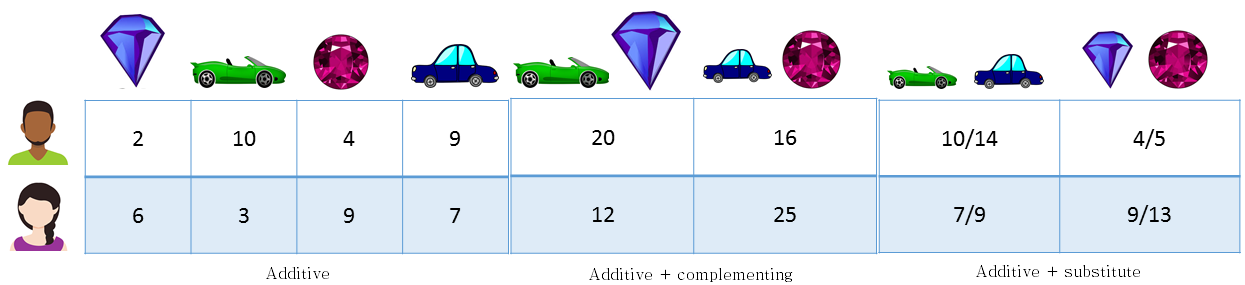
\includegraphics[width=7in]{images/utilities.png}\Description{Additive, complementary and substitute utilities}
% \caption{Additive, complementing, and substitute values in Inheritance distribution}
% \end{figure*}

\subsection{Additive goods and utilities}
Formally, additive goods/utilities are the ones who showcase mathematical additive properties. Additive goods are the ones whose utility is independent of others. Additive utilities are same as the one specified in previous section; that is, for agent $i$, the additive utility function is $V_i: \mathcal{M} \rightarrow \mathbb{R_+}$. Total utility of a set of goods/allocations is equal to the sum of all disjoint subsets.
\[
    U_i = \sum_{a \in \mathcal{A}_i} V_{i,a}
\]

Where $\mathcal{A}_i$ is the allocation of goods to agent $i$ and $V_{i,a}$ is agent $i$'s value for good $a$.

\subsection{Complementary goods and utilities}
\label{section_complementary}

Two goods are said to be complements if demand for one show similarity with the demand for other. In other words, their demands are linked in such a way that increase in one raises the demand of the other, and same with the decrease in demand. A popular real-world example of complementary goods is razors blades. If the sell of razors increases, the demand for blades will rise too. This is an example of perfect complements. One can't use razors without blades or the other way, blades without razors. Real-world is full of such examples; burger and fries, hot dogs and buns, cars and gas, etc. Some of them are perfect complements, others are not.

In this paper, we define complements over pairs of adjacent goods. We denote complementing valuation for each agent $i$ as: 

\[
    C_i: \frac{\mathcal{M}}{2} \rightarrow \mathbb{R_+}
    % v_i: \forall_{j < |M|/2} (M_{2j}, M_{2j+1})\mapsto \mathbb{R_+}
\]

An agent will earn the complementing utility if its allocation contains both the goods representing that value, otherwise not. If it does, it will be added to the overall valuation of the set of goods which may include additive evaluations of each of the individual goods in the set.

For some set of goods $G$, and given agent $i$'s additive values for each good $l \in G$, $V_{i,l}^{add}$ and complementing values for pairs of goods $\{2l, 2l+1\} \in G$ , $V_{i,l}^{com}$
\[
    V_i(G) = \sum_{l=1}^m \mathbbm{1}_{l \in G}V_{i,l}^{add} + \sum_{l=1}^{m/2} \mathbbm{1}_{\left(2l,2l+1\right) \in G}V_{i,l}^{com}
\]

\begin{figure}
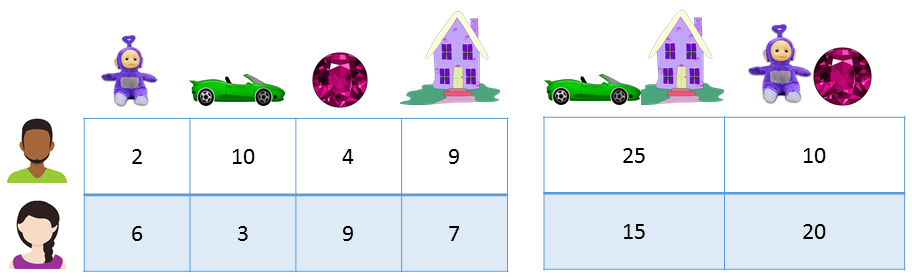
\includegraphics[width=3in]{images/complementary_values.png}\Description{Additive and complementing values in inheritance distribution}
\caption{Additive and complementing utilities in inheritance allocation}
\label{fig_inherit_compl_val_ex}
\end{figure}

Figure \ref{fig_inherit_compl_val_ex} shows an example of inheritance distribution problem. Here, each agent has some additive utility for some object in the inheritance. It also has complementing utility over pairs of goods showing the value of goods if allocated together. In this example, one of the agent might be an old person who really needs a car and a house, so has a higher utility for the combination; while the other might be a young person who prefers a family heirloom toy and a precious jewellery.

\subsection{Substitute goods and utilities}
\label{section_substitute}

Two goods are said to be substitutes if demand for one show reverse dependency on the demand of other. In other words, their demands are linked in such a way that increase in one decreases the demand of the other, and similarly the other way. A real-world example of substitute goods is potatoes from two farms. If the cost of potatoes from one farm increases, the demand of potatoes from another similar farm with cheaper price will increase. With increase in demand, the price of potatoes from the other farm will increase too. If the potatoes from two farms are exactly similar, this is called a perfect substitute. In perfect substitutes, one can easily replace one good with the other and having both does not improve the utility. Some real-world examples of substitute goods are; bike and car, farms, tea and coffee, pencils and pens, etc. Some of them are perfect substitutes, others are not.

We define two types of substitutes over pairs of adjacent goods: type 1 and type 2.

Type 1 substituting utilities for agent $i \in \mathcal{N}$ is
\[
    S^1_i:  \frac{\mathcal{M}}{2} \rightarrow \mathbb{R_+}
\]
\[
    S^1_{i,l} = min(U_{i,2l}, U_{i, 2l+1}) \quad \forall l < |\mathcal{M}|/2
\]

Type 2 substituting utilities for agent $i \in \mathcal{N}$ is
\[
    S^2_i:  \frac{\mathcal{M}}{2} \rightarrow \mathbb{R_+}
\]
\[
    S^2_{i,l} = rand(0, min(U_{i,2l}, U_{i,2l+1})) \quad \forall l < |\mathcal{M}|/2
\]

An agent will earn the substitute utility if its allocation contains both the goods representing that value, otherwise not. If it does, it will be subtracted from the additive utility to get the total utility of the allocation of agent $i$.

For some set of goods $G$, and given agent $i$'s additive values for each good $l \in G$, $V_{i,l}^{add}$ and substituting values for pairs of goods $\{2l, 2l+1\} \in G$ , $V_{i,l}^{sub^{1/2}}$
\[
    V_i(G) = \sum_{l=1}^m \mathbbm{1}_{l \in G}V_{i,l}^{add} - \sum_{l=1}^{m/2} \mathbbm{1}_{\left(2l,2l+1\right) \in G}V_{i,l}^{sub^{1/2}}
\]

\begin{figure}
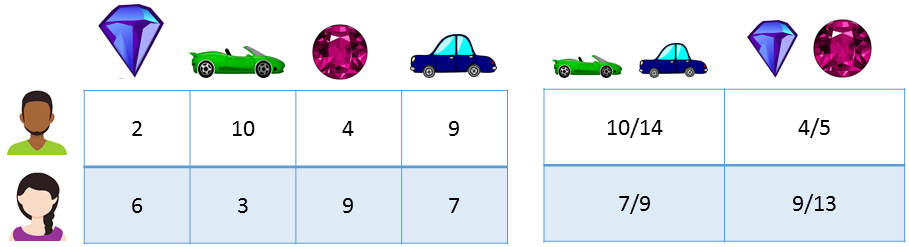
\includegraphics[width=3in]{images/substitute_values.png}\Description{Additive and substituting values in inheritance distribution}
\caption{Additive and substitute (type 1/type 2) utilities in inheritance allocation}
\label{fig_inherit_subst_val_ex}
\end{figure}

Figure \ref{fig_inherit_subst_val_ex} shows an example of inheritance distribution problem with substitute goods. Each agent has some additive value over individual goods in the inheritance. In addition to that, goods like cars show substituting utility, that is, the value of a pair combined may not be equal to sum of value of each goods individually. This means trying to get two cars instead of one car and one precious jewellery may not be a wise idea as two cars forms a substitute goods and may have lesser combined value.


\subsection{Fairness, Envy, and Envy-freeness}
\label{section_envy}
Fairness is one of the primary criteria in any resource allocation problem. The notion of fairness differs with the definition of the allocation problem. Consider the problem of division of a cake among $n$ people. Each person should receive $n$th part of the cake. We extend the problem by starting with $m$ cakes. Share of each person should now be $m/n$. The fairness criterion here is very loose as the only constraint we are trying to satisfy is equal distribution among all. In the same problem, we introduce the concept of age of a person. A person should receive a portion of a cake with respect to the age. Young ones would get more cake than the older. The fairness criteria now is to strictly get more cake if younger and not necessarily equal if same age. The criteria can further be varied by introducing different types of food and preferences of people over the types of food.

One fairness criterion studied extensively in literature is envy-freeness. Envy is defined as an amount with which an agent prefers an allocation of someone else. 

\begin{definition}{Envy}
\label{def_envy}
An agent $i$ with a value of $v_{ia}$ for a good $a$ which is allocated to agent $j$ who has a value of $v_{ja}$ for the same good $a$ envies agent $j$ by an
amount $e_{ij} = v_{ja} - v_{ia}$. The entity $e_{ij} \geq 0$ implies agent $i$ does not envy agent $j$, whereas $|e_{ij}|$ is the amount of envy $i$ has for $j$ otherwise. Extending the same to the entire allocation $\mathcal{A}_i$ instead of a single good, $E_{ij} = V_i(\mathcal{A}_j) - V_i(\mathcal{A}_i)$, where $V_i$ is the value function for agent $i$, and $\mathcal{A}_i$ and $\mathcal{A}_j$ are allocations of $i$ and $j$, respectively.
\end{definition}

Envy-freeness (EF) is a notion of fair allocation where every agent prefers their own allocation over that of any other agent. In other words, every agent feels their allocation is better than or at least as valuable as the allocation of any other agent.


\begin{definition}{Envy-freeness (EF)}
\label{def_envyfree}
An allocation is envy-free if $\mathcal{A}_i \succeq_i \mathcal{A}_j \forall i,j$ where $\mathcal{A}_i$ and $\mathcal{A}_j$ is the allocation of $i$ and $j$, respectively. Given a value function $V_i$ for agent $i$, $V_i(\mathcal{A}_i) \geq V_i(\mathcal{A}_j)$ $\forall i,j$. 
\end{definition}

For a simple cake division problem, each person would want a piece of size greater than or at least equal to any other person. No one would want to exchange their piece with anyone else. This results in everyone having same sized pieces of the cake.

In the extended version of the problem, the idea of envy should reflect the age of the person. In an envy-free allocation, each person will have a piece of cake according to their own age and ensuring the fact that they don't want the piece of any other person. 

Fair distribution of a cake is an example of divisible goods. There always exist an envy-free solution for the allocation of divisible goods \cite{stern1958puzzle}. Though, increasing the number of agents, increases the complexity of the envy-free allocation and it may take a very long time for computation \cite{aziz2016discrete}.

The problem gets difficult for indivisible goods. In a simple example with one item and two agents, where both have positive utilities for the item, the item can only be allocated to one of the agents. No matter which agent gets the item, the other agent will always envy for not getting the item. Envy-free division can not be guaranteed in general for the case of indivisible goods. The problem of determining whether an allocation exists, which is envy-free, is a computationally difficult (NP-complete) problem \cite{lipton2004approximately}. Additionally, optimality constraint (such as Pareto efficiency) makes the problem NP-hard \cite{bouveret2008efficiency}.

For feasibility, we weaken the constraint on envy-freeness and attempt allocation under these constraint.

\begin{definition}{Envy-free up to one good (EF1) \cite{caragiannis2016unreasonable}}
\label{def_ef1}
An allocation $\mathcal{A}$ is envy-free up to one good (EF1) if for all agents $i$, $j$, agent $i$ will stop envying agent $j$ if a good $g$, for some $g$ in $\mathcal{A}_j$ is dropped from the allocations of agent $j$, $\mathcal{A}_j$. Formally,
$$
    \forall i,j \in \mathcal{N}, \exists g \in \mathcal{A}_j, V_i(\mathcal{A}_i) \geq V_i(\mathcal{A}_j \backslash \{g\})
$$
\end{definition}

We further relax the envy-freeness fairness criterion for up to $k$ goods.

\begin{definition}{Envy-free up to $k$ goods (EFk).}
\label{def_efk}
An allocation $\mathcal{A}$ is envy-free up to $k$ goods (EFk) if for all agents $i$, $j$, agent $i$ will stop envying agent $j$ if a set of goods $\mathcal{G} \subseteq \mathcal{A}_j$, such that $|\mathcal{G}| = k$, is dropped from the allocations of agent $j$, $\mathcal{A}_j$. Formally,
$$
    \forall i,j \in \mathcal{N}, k \leq |\mathcal{M}|, \exists G \subseteq \mathcal{A}_j, |G| = k, V_i(\mathcal{A}_i) \geq V_i(\mathcal{A}_j \backslash \{G\})
$$
\end{definition}

In other words, if agent $i$ doesn't envy agent $j$ once we drop some $k$ goods from agent $j$'s allocation $\mathcal{A}_j$, then the allocation is called envy-free up to $k$ goods (EFk).

Also, the definition \ref{def_efk} allows an EFk allocation to be EF(k+1), EF(k+2), and so on, as once we have an EFk allocation $ \exists G \subseteq \mathcal{A}$, $ |G|=k \ni V_i(\mathcal{A}_i) - V_i(\mathcal{A}_j \backslash G) \geq 0 $ and dropping more goods from agent $j$'s allocation would only increase $V_i(\mathcal{A}_i) - V_i(\mathcal{A}_j \backslash G)$ and not create any new envy.


\subsection{Welfare and Maximum Nash Welfare}
\label{section_welfare}
Welfare is a concept of an economic system which measures happiness and well-being of all the participating agents with some agreed definition of happiness or well-being. It follows the idea of fairness from the previous section. A system which is fair to all the constituting members can be said to ensure the welfare of all the participants, and further, the welfare of the entire system. We adopt the terminology of welfare in the resource allocation problem. Given an allocation of goods among agents, we believe we have achieved welfare if we have a fair allocation for each agent.

Like fairness, the notion of welfare differs with the definition of the resource allocation problem. Following the example from the previous section, for the simple cake division problem, equal division of cake among all agents would achieve the welfare in cake distribution. In the extended version of the cake division problem, if each agent receives a fair amount of cake based on the fairness criterion of age, the division will ensure welfare of the system.

Three popular notions of welfare are often discussed in economics: utilitarian, egalitarian and Nash.

An utilitarian welfare strives to achieve maximum overall utility. In resource allocation problem, a good will be allocated to that agent who has the maximum value for it. This ensures the maximum possible usage of the goods. Here, the idea of fairness is specified as maximum utilization of the goods. In that sense, it provides the most efficient allocation. Utilitarian distribution does not ensure that each agent receive some good. An agent who does not have the best value for any good, may not get any good. Also, it is possible that one may have best value for all of the goods and may end up receiving all the goods. In other words, utilitarian welfare, in trying to achieve the highest possible utility, does not ensure positive utility for all the participants.

An egalitarian welfare tries to maximize well-being or happiness of all agents. It strives to achieve equality of some type among all agents. In resource allocation problem, an egalitarian welfare system would not regard the utilities that agents have for various goods. A good should be allocated to an agent who owns the least amount. With a notion of equality defined, an egalitarian welfare provides the most fair allocation.

The simple cake division problem described above is both utilitarian and egalitarian. Every agent gets an equal share of the cake, and since every agent have the same value for the cake, the distribution achieves maximum efficiency. For the extended version of the cake division problem, the value for the cake is inversely proportional to the age of the person. The egalitarian welfare solution would allocate an equal amount of cake to everyone, whereas the utilitarian welfare solution would distribute cake based on the value.

The maximum Nash welfare (MNW) solution provides both fairness and efficiency. We follow the definition the MNW solution by \citet{caragiannis2016unreasonable}

\begin{definition}{Nash welfare (NW) or Nash product} \label{def_nw}
Nash welfare or Nash product is a product of utilities of agents for allocated goods with a condition that every agent values it's allocation positively

\begin{equation}
    NW(\mathcal{A}) = 
    \begin{cases}
    \prod_{i \in \mathcal{N}} V_i(\mathcal{A}_i), & \text{if } \forall i \in \mathcal{N}, V_i(\mathcal{A}_i) > 0 \\
    \text{not defined}, & \text{otherwise}
    \end{cases}
\end{equation}

for all agents $i$ in $\mathcal{N}$, where $V$ is the value function and $\mathcal{A}$ is the allocation.
\end{definition}

\begin{definition}{Maximum Nash welfare (MNW).} \label{def_mnw}
MNW allocation is the one that maximizes the Nash welfare among all possible allocations

$$
    \mathcal{A}^{MNW} = \operatorname{arg\,max}_{A \in \prod_{|\mathcal{N}|}(\mathcal{M})} NW(\mathcal{A})
$$
\end{definition}


Maximum Nash welfare is widely known for its welfare guarantees. MNW is found to satisfy interesting properties in a fair allocation problem. MNW is efficient, satisfying Pareto optimality, and it has an attractive fairness property in the form of envy-freeness.

Pareto optimal (PO) allocation is the one in which it is not possible to make allocations of one agent better without making another agent's allocation worse. PO is used as a property of efficient allocations because an allocation will not be Pareto if one can find an alternate allocation which improves the welfare for at least one agent without hurting the welfare of any other agent. With existence of no such improvement, PO represents the best possible scenario under such efficiency preference criteria.

\begin{definition}{Pareto optimality (PO).}
An allocation $\mathcal{A}$ is Pareto optimal if no other allocation $\mathcal{A'}$ is feasible such that $V_i(\mathcal{A}_i') \geq V_i(\mathcal{A}_i)$ for all agents $i \in \mathcal{N}$ with $ V_j(\mathcal{A}_j') > V_j(\mathcal{A}_j)$ for some agent $j \neq i$ where, $V_i$ is the value function for any agent $i \in \mathcal{N}$.
\end{definition}

\begin{theorem}
Every MNW allocation of indivisible goods is Pareto optimal (PO).
\end{theorem}

\begin{proof}
We follow a simple proof of Pareto optimality for MNW by \citet{caragiannis2016unreasonable}. It is trivial for every MNW allocation $\mathcal{A}$ to be PO because any alternate allocation $\mathcal{A}'$ that increases the utility of one agent without decreasing the utility of any other agent would result in increase in the Nash welfare of the alternate allocation $\mathcal{A}'$, that is $NW(\mathcal{A}') > NW(\mathcal{A})$, contradicting the assumption that the original MNW allocation $\mathcal{A}$ had the maximum/optimal NW of all the possible allocations. 
\end{proof}

Maximum Nash welfare allocations also satisfy the elusive fairness property of envy-freeness (EF) defined in the previous section. This is further studied and proved in the next section.

With PO and EF, the maximum Nash welfare, in a great degree of simplicity, is one of the rare algorithms providing us with both efficiency and fairness standards. It is a good balance between the utilitarian vs. egalitarian trade-off. Also, attempting to maximize for utilitarian or egalitarian welfare conditions results in non-EF allocations \cite{caragiannis2016unreasonable}. In that sense, MNW allocation prevails over utilitarian and egalitarian allocation criteria for the strong PO and EF guarantees that it ensures.

% End of section 3 ----------------------------------------------------------

\section{Experiments}
\label{section_experiments}

% Maximum Nash Welfare computation - value function abstracted
\begin{algorithm}
\caption{ Computing an MNW allocation }
\label{algorithm1}
\SetAlgoLined
\KwIn{ Agents $\mathcal{N}$, resources $\mathcal{M}$, value function $value\_f$, additive utilities $AU$, complementary/substituting utilities $CSU$ }
\KwOut{ An MNW allocation $ \mathcal{A}^{MNW}$ }
 $Max\_NW \leftarrow 0 $ \;
 $\mathcal{A}_{Max\_NW} \leftarrow \phi $ \;
 \For{all possible allocations $ \mathcal{A} (N \times M) $}{
  $NW_\mathcal{A} \leftarrow \prod_{i \in \mathcal{N}} value\_f(\mathcal{A}_i, AU, CSU) $ \;
  \If{$NW_{\mathcal{A}} > Max\_NW $}{
   $Max\_NW \leftarrow NW_{\mathcal{A}}$ \;
   $\mathcal{A}_{Max\_NW} \leftarrow \mathcal{A} $ \;
  }
 }
\end{algorithm}

% Nash Welfare/Product computation
% For additive, complementing, substituting (type 1 and 2) utilities
\begin{algorithm}
\caption{ Computing Nash welfare }
\label{algorithm2}
\SetAlgoLined

Pairwise Allocation: \\
$ PA = (\mathcal{A}) \rightarrow [min(\mathcal{A}_{i,2j}, \mathcal{A}_{i,2j+1}) \forall i \in \mathcal{N}, j < |\mathcal{M}|/2] $

\BlankLine

Substituting utilities - type 1: \\
$ SU_1 = (AU) \rightarrow [min(AU_{i,2j}, AU_{i,2j+1}) \forall i \in \mathcal{N}, j < |\mathcal{M}|/2] $

\BlankLine

Substituting utilities - type 2: \\
$ SU_2 = (AU) \rightarrow [rand(0, min(AU_{i,2j}, AU_{i,2j+1})) \forall i \in \mathcal{N}, j < |\mathcal{M}|/2] $

\BlankLine
\BlankLine

$ NW_{additive} = (\mathcal{A}, AU) \rightarrow \mathcal{A} \cdot AU $

$ NW_{compl} = (\mathcal{A}, AU, CU) \rightarrow \mathcal{A} \cdot AU + PA(\mathcal{A}) \cdot CU $

$ NW_{subst1} = (\mathcal{A}, AU) \rightarrow \mathcal{A} \cdot AU - PA(\mathcal{A}) \cdot SU_1(AU) $

$ NW_{subst2} = (\mathcal{A}, AU) \rightarrow \mathcal{A} \cdot AU - PA(\mathcal{A}) \cdot SU_2(AU) $

\end{algorithm}

In this section, we describe the data, computations, and analysis of the features of the data.

We simulate the problem with $n = 2$ agents competing for allocation of $m$ goods where $m \in \{10, 8, 6, 4\}$. Each agent has some value for each of the goods. We generate $m$ random independent and identically distributed (IID) numbers over $[0, 100)$ to represent additive valuations of an agent for $m$ goods. We further generate $m/2$ random IID numbers over $[0, 100)$ representing agent's valuation for pairs of complementing goods. Each complementing utility represents the collective value an agent would receive if both the goods are allocated to the agent.

We further compute substitute utilities of type 1 and type 2 based on the additive utilities of the goods as defined in algorithm \ref{algorithm2}. As with complementing utilities, both of these represent the collective value an agent would get if the pair of goods is allocated to the agent.

To sum up, we have four types of utility valuation, namely i) Additive ii) Complementing iii) Substituting type 1 iv) Substituting type 2. We generate 1000 samples for each $m \in \{10, 8, 6, 4\}$ and store it for reproducibility. MNW is computed for each of these sample with respect to four types of valuations with algorithm \ref{algorithm1}.

% Discussion on analysis of experiements starts here

% Percent EFness
\begin{figure}[h!]
    \centering
    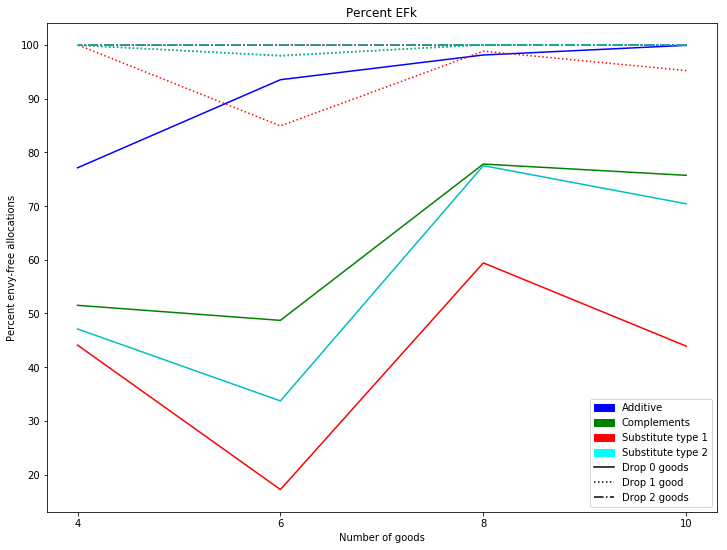
\includegraphics[width=\linewidth]{images/ef_percent.png}
    \caption{Percent EFk}
    \label{fig_efk_perc}
    \small
        Percent MNW allocations satisfying EF0, EF1, and EF2, respectively for additive, complementing, substituting type-1, substituting type-2 utilities.
\end{figure}

Figure \ref{fig_efk_perc} shows the percent of samples which satisfies the envy-freeness criteria. Simple additive utilities gradually creates lesser envy with the increase in the number of goods. It also provides the experimental proof for envy-freeness up to one good (EF1) property of MNW allocations with additive valuations \cite{caragiannis2016unreasonable}. Figure \ref{fig_efk_perc} indicates pairwise complementing and substituting valuations are envy-free up to 2 goods (EF2). Complementing and substituting utilities also showcase surprisingly high, but not perfect, EF1. In particular, substituting type-1 utilities for 4 goods and type-2 for 10, 8, and 4 goods have 100\% EF1.


% Mean Envy
\begin{figure}[h!]
  \centering
  \begin{subfigure}[b]{\linewidth}
    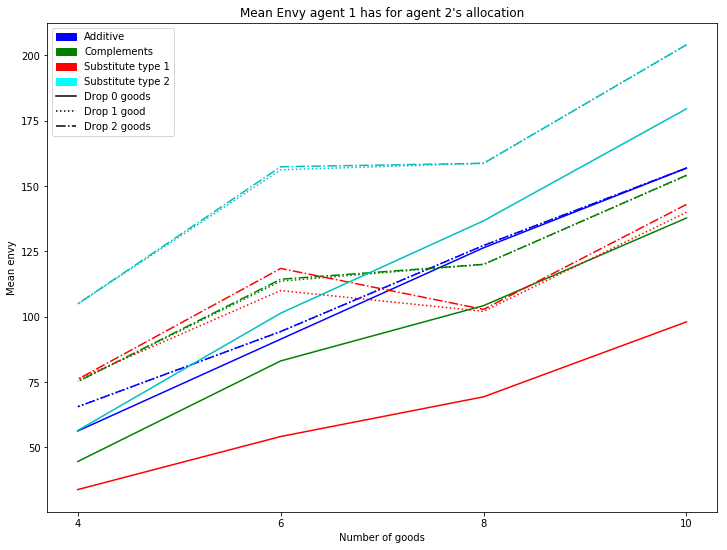
\includegraphics[width=\linewidth]{images/mean1_2.png}
    \caption{}
  \end{subfigure}
  \begin{subfigure}[b]{\linewidth}
    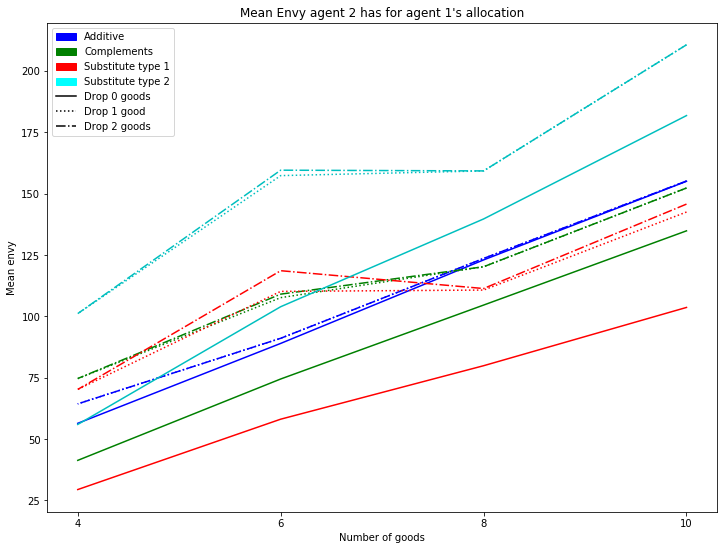
\includegraphics[width=\linewidth]{images/mean2_1.png}
    \caption{}
  \end{subfigure}
  \caption{Mean envy}
  \label{fig_efk_mean}
  \small
    Mean envy present in MNW allocations after dropping 0, 1, and 2 goods, for additive, complementing, substituting type-1, substituting type-2 utilities. (a) Agent 1's mean envy for agent 2's allocation (b) Agent 2's mean envy for agent 1's allocation
\end{figure}

Figure \ref{fig_efk_mean} plots mean envy between the agents after dropping 0, 1, and 2 goods for all MNW allocations. Mean envy-freeness raises with drops of 0, 1 and 2 goods as expected. The difference is greater from EF0 to EF1 than from EF1 to EF2 which is almost the same. This indicates when agents drop the first good in EF1 calculation, though it is known to drop the one which is valued the most by others, the first drop has a very high utility.


% Mean Positive/Negative Envy
\begin{figure}[h!]
  \centering
  \begin{subfigure}[b]{\linewidth}
    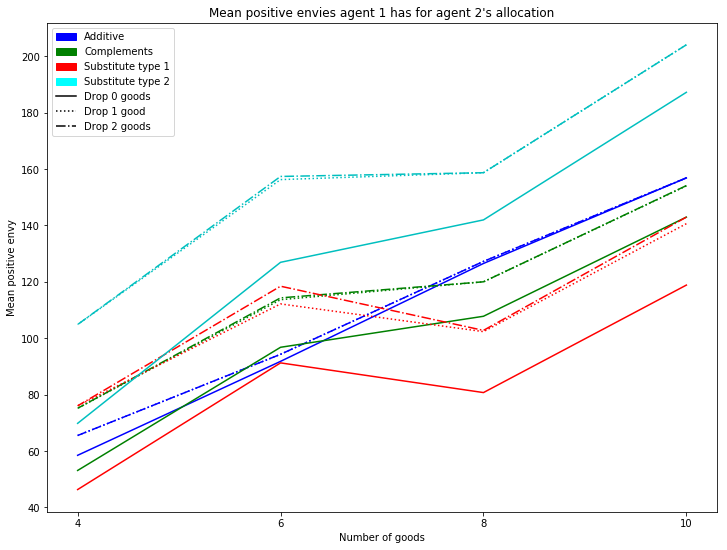
\includegraphics[width=\linewidth]{images/mean1_2pos.png}
    \caption{}
  \end{subfigure}
  \begin{subfigure}[b]{\linewidth}
    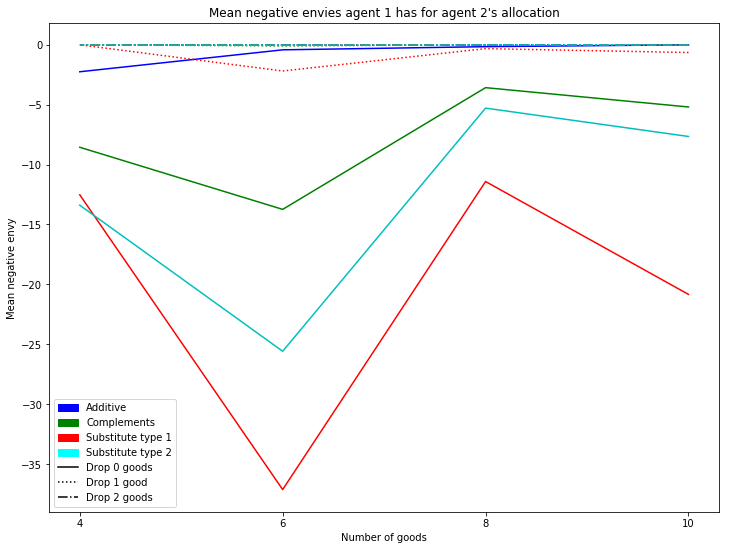
\includegraphics[width=\linewidth]{images/mean1_2neg.png}
    \caption{}
  \end{subfigure}
  \caption{Mean positive and negative envy}
  \label{fig_efk_meanpn}
  \small
    Mean (a) positive (non-envy) and (b) negative (envy) envy present in MNW allocations after dropping 0, 1, and 2 goods for additive, complementing, substituting type-1, substituting type-2 utilities. We only show agent 1's positive/negative envy for agent 2's allocation as the reverse show approximately same pattern.
\end{figure}

Figure \ref{fig_efk_meanpn} plots the mean positive and negative envy in the allocations after dropping 0, 1, and 2 goods for EF0, EF1, and EF2, respectively. Mean positive envy (non-envy) closely follows and reflects the figure \ref{fig_efk_mean} mean envy plot. Mean negative envy plot reflects association with figure \ref{fig_efk_perc} - percent EFk. It is the plot of envy values for the agents who negatively envies other agents. Similar to figure \ref{fig_efk_perc}, EF2 shows zero envy. The same high EF1 pattern as figure \ref{fig_efk_perc} is visible in figure \ref{fig_efk_meanpn} with some allocations showing zero negative envy.


% DFs additive
\begin{figure}[h!]
  \centering
  \begin{subfigure}[b]{0.47\linewidth}
    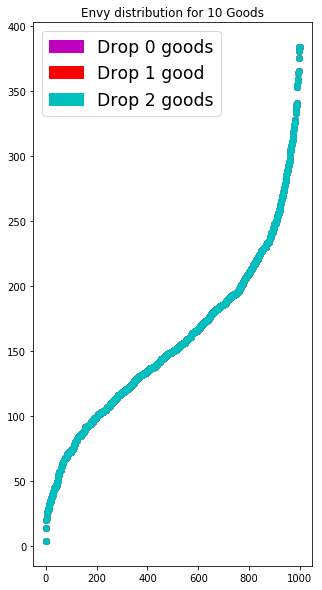
\includegraphics[width=\linewidth]{images/envy_density/envy_density_u10.png}
    \caption{}
  \end{subfigure}
  \begin{subfigure}[b]{0.47\linewidth}
    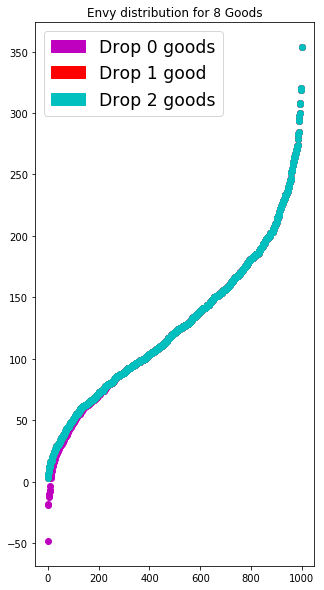
\includegraphics[width=\linewidth]{images/envy_density/envy_density_u8.png}
    \caption{}
  \end{subfigure}
  \begin{subfigure}[b]{0.47\linewidth}
    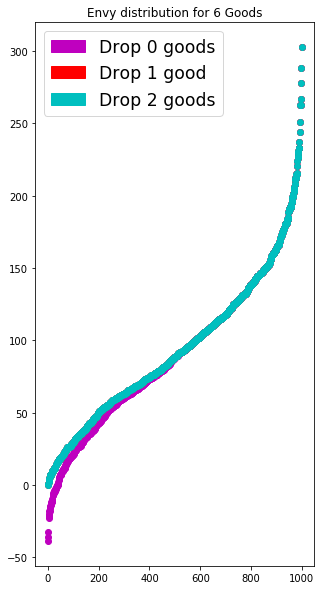
\includegraphics[width=\linewidth]{images/envy_density/envy_density_u6.png}
    \caption{}
  \end{subfigure}
  \begin{subfigure}[b]{0.47\linewidth}
    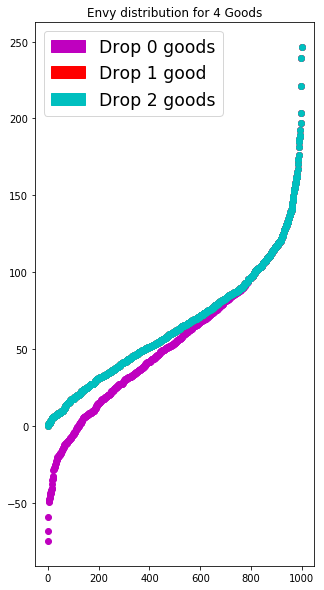
\includegraphics[width=\linewidth]{images/envy_density/envy_density_u4.png}
    \caption{}
  \end{subfigure}
  \caption{Envy distribution curve - Additive Utilities}
  \label{fig_efk_dist_curve_add}
  \small
    Envy distribution of the entire sample space with additive utilities after dropping 0, 1, and 2 goods for number of goods (a) $m = 10$, (b) $m = 8$, (c) $m = 6$, (d) $m = 4$
\end{figure}

% DFs complementing
\begin{figure}[h!]
  \centering
  \begin{subfigure}[b]{0.47\linewidth}
    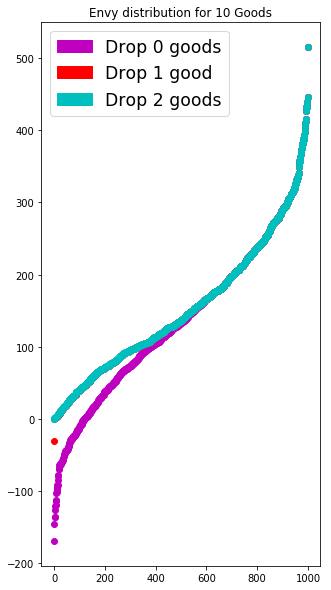
\includegraphics[width=\linewidth]{images/envy_density/envy_density_uv10.png}
    \caption{}
  \end{subfigure}
  \begin{subfigure}[b]{0.47\linewidth}
    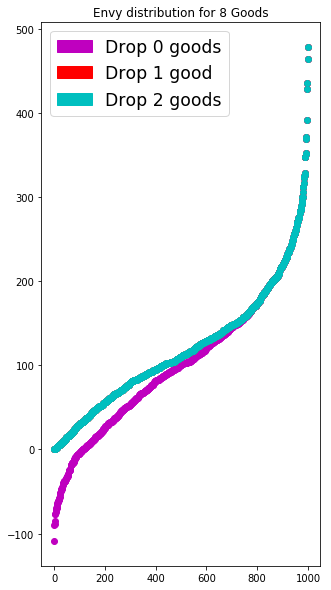
\includegraphics[width=\linewidth]{images/envy_density/envy_density_uv8.png}
    \caption{}
  \end{subfigure}
  \begin{subfigure}[b]{0.47\linewidth}
    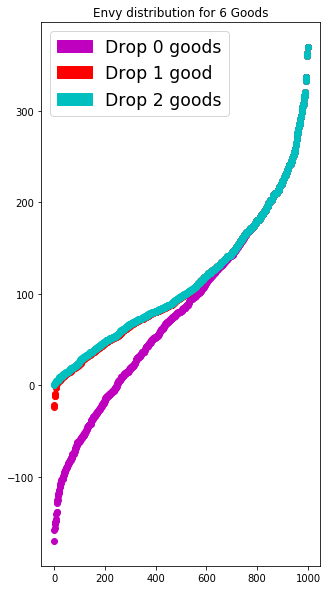
\includegraphics[width=\linewidth]{images/envy_density/envy_density_uv6.png}
    \caption{}
  \end{subfigure}
  \begin{subfigure}[b]{0.47\linewidth}
    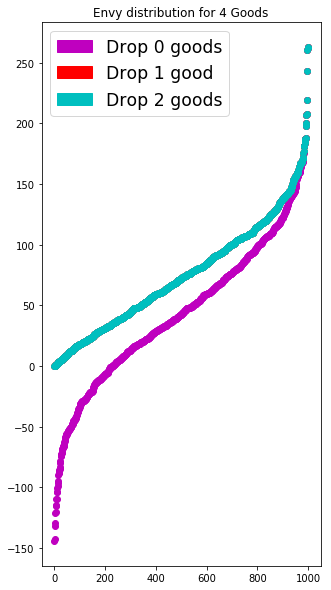
\includegraphics[width=\linewidth]{images/envy_density/envy_density_uv4.png}
    \caption{}
  \end{subfigure}
  \caption{Envy distribution curve - Complementing Utilities}
  \label{fig_efk_dist_curve_compl}
  \small
    Envy distribution of the entire sample space with complementing utilities after dropping 0, 1, and 2 goods for number of goods (a) $m = 10$, (b) $m = 8$, (c) $m = 6$, (d) $m = 4$
\end{figure}

% DFs substituting type-1
\begin{figure}[h!]
  \centering
  \begin{subfigure}[b]{0.47\linewidth}
    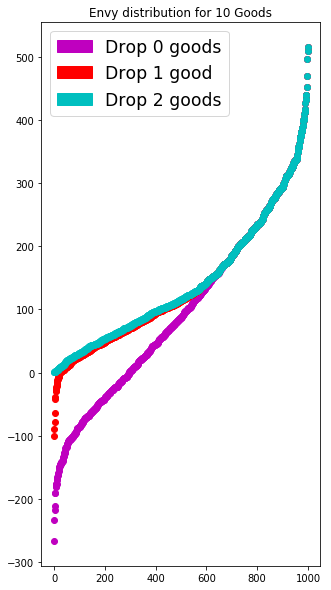
\includegraphics[width=\linewidth]{images/envy_density/envy_density_us19.png}
    \caption{}
  \end{subfigure}
  \begin{subfigure}[b]{0.47\linewidth}
    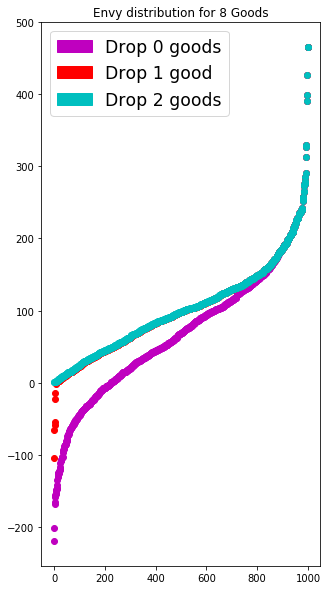
\includegraphics[width=\linewidth]{images/envy_density/envy_density_us18.png}
    \caption{}
  \end{subfigure}
  \begin{subfigure}[b]{0.47\linewidth}
    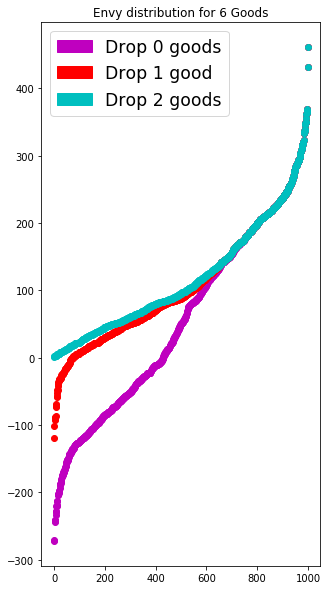
\includegraphics[width=\linewidth]{images/envy_density/envy_density_us16.png}
    \caption{}
  \end{subfigure}
  \begin{subfigure}[b]{0.47\linewidth}
    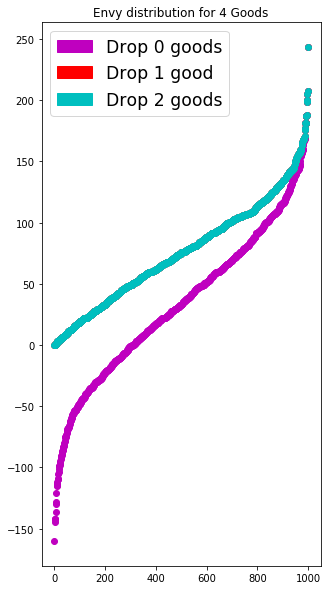
\includegraphics[width=\linewidth]{images/envy_density/envy_density_us14.png}
    \caption{}
  \end{subfigure}
  \caption{Envy distribution curve for Substituting type 1 Utilities}
  \label{fig_efk_dist_curve_subst1}
  \small
    Envy distribution of the entire sample space with substituting utilities type 1 after dropping 0, 1, and 2 goods for number of goods (a) $m = 10$, (b) $m = 8$, (c) $m = 6$, (d) $m = 4$
\end{figure}

% DFs substituting type-2
\begin{figure}[h!]
  \centering
  \begin{subfigure}[b]{0.47\linewidth}
    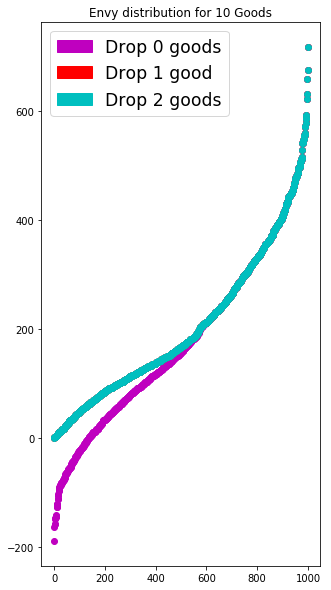
\includegraphics[width=\linewidth]{images/envy_density/envy_density_us29.png}
    \caption{}
  \end{subfigure}
  \begin{subfigure}[b]{0.47\linewidth}
    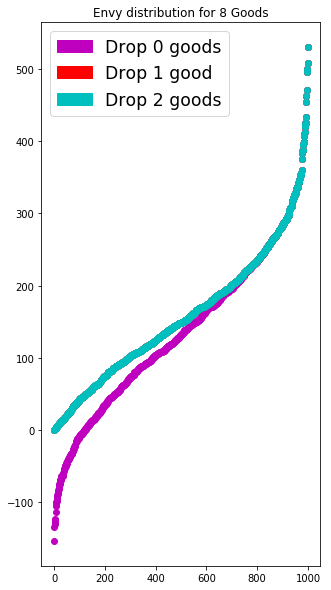
\includegraphics[width=\linewidth]{images/envy_density/envy_density_us28.png}
    \caption{}
  \end{subfigure}
  \begin{subfigure}[b]{0.47\linewidth}
    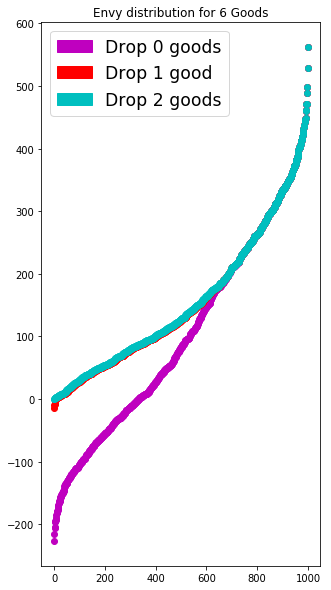
\includegraphics[width=\linewidth]{images/envy_density/envy_density_us26.png}
    \caption{}
  \end{subfigure}
  \begin{subfigure}[b]{0.47\linewidth}
    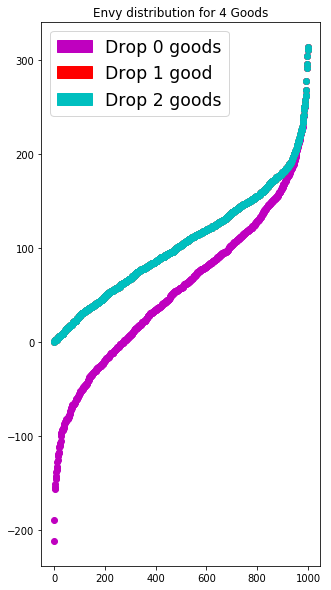
\includegraphics[width=\linewidth]{images/envy_density/envy_density_us24.png}
    \caption{}
  \end{subfigure}
  \caption{Envy distribution curve for Substituting type 2 Utilities}
  \label{fig_efk_dist_curve_subst2}
  \small
    Envy distribution of the entire sample space with substituting utilities type 2 after dropping 0, 1, and 2 goods for number of goods (a) $m = 10$, (b) $m = 8$, (c) $m = 6$, (d) $m = 4$
\end{figure}


Figure \ref{fig_efk_dist_curve_add}-\ref{fig_efk_dist_curve_subst2} plot the distributions of envy for simulated 1000 samples. The decrease in number of goods reflects in increase in number of envied allocations. These curves give a nice shape to the envy calculations before and after dropping goods for EF0, EF1, and EF2 calculations. Figure \ref{fig_efk_dist_curve_add}-\ref{fig_efk_dist_curve_subst2} show both, final envy which is sorted on the sampling x-axis which forms a smooth shape with rest of the non-envying distribution curve.

% End of section 4 ----------------------------------------------------------

\section{MNW and EFk}
\label{section_proof}

In this section, we analyze the relation between maximum Nash welfare and envy-freeness up to k goods.

We already know MNW allocations for additive utility values are envy-free up to one good (EF1) \cite{caragiannis2016unreasonable}. The experiments on goods with additive utilities in previous section provide the experimental evidence to that fact.

In previous section, we conduct experiments on complementary and substitute goods. We have simulated the complements and substitutes of the goods in the market in terms of the dependency of utility valuation for pairs of goods. An interesting fact emerge from the plots is that, all of the MNW allocations are envy-freeness up to 2 goods.

We formally define the value of a set of goods $G$ which is part of a larger allocation of an agent $i$, $\mathcal{A}_i$ as below.

\begin{definition}{Value of goods given an allocation (W).}
\label{def_dep_value}
The value $W_i(G | \mathcal{A}_i)$ of a set of goods $G$ for an agent $i \in \mathcal{N}$ given the allocation of the agent $i$, $\mathcal{A}_i$ is equal to the sum of the additive valuation of each good $g \in G$, collective valuation of dependencies $C \subseteq G$, and valuation of dependency that goods $G' \subseteq G$ may form with any set of goods $A' \subseteq \mathcal{A}_i$.
\end{definition}

\subsection{Pairwise complements and EF2}
\label{subsection_EF2_compl}

Extending the idea of EF1 of additive goods \cite{caragiannis2016unreasonable}, in this section, we formally state an envy-freeness criteria for goods with pairwise complementing values.

\begin{theorem}
Every MNW allocation is envy-free up to 2 goods (EF2) for goods which show additive and complementing valuations based on the pair of adjacent goods.
\end{theorem}

\begin{proof}
We approach this proof by contradiction. We start with a MNW allocation $\mathcal{A}$ being not EF2, so that agent $i$ envies agent $j$ even after removing 2 goods from agent $j$'s allocation $\mathcal{A}_j$

Following section \ref{section_complementary}, the value of a set of goods $G$ for agent $i$ showing pairwise complementing utilities is given by

\[
    V_i(G) = \sum_{l=1}^m \mathbbm{1}_{l \in G}V_{i,l}^{add} + \sum_{l=1}^{m/2} \mathbbm{1}_{\left(2l,2l+1\right) \in G}V_{i,l}^{com}
\]

where $V_{i,l}^{add}$ is the additive utility, $AU$ of agent $i \in \mathcal{N}$ for good $l \in \mathcal{M}$ allocated in $G$; $V_{i,l}^{com}$ is the complementing utility, $CU$ of agent $i \in \mathcal{N}$ for an adjacent pair of goods $\{2l,2l+1\} \in \mathcal{M}$ allocated in $G$.

Let such pairs of goods be represented as $G = \{l_x, l_y\}$.

Let $\mathcal{A}'$ denote the allocation obtained by moving a pair of good $\{l_x, l_y\}$ from agent $j$ to agent $i$ in $\mathcal{A}$. So, $\mathcal{A}_i' = \mathcal{A}_i \cup \{l_x, l_y\} $ and $\mathcal{A}_j' = \mathcal{A}_j\backslash \{l_x, l_y\}$.

The value of the pair of goods $G = \{l_x, l_y\}$ for agents $i$ given its allocations $\mathcal{A}_i$ is

\begin{equation}
\label{eq_val_given_alloc_compl}
    W_i(G=\{l_x,l_y\} | \mathcal{A}_i) = 
    \begin{gathered}
        V_{i,l_x}^{add} + V_{i,l_y}^{add} \\
        + \mathbbm{1}_{l_{x \pm 1} \in \mathcal{A}_i}V_{i,l_{x,x\pm 1}}^{com} \\
        + \mathbbm{1}_{l_{y \pm 1} \in \mathcal{A}_i}V_{i,l_{y,y\pm 1}}^{com} \\
        + \mathbbm{1}_{l_y = l_{x \pm 1}}V_{i,l_{x,y}}^{com}
    \end{gathered}
\end{equation}

In other words, by definition \ref{def_dep_value}, the value of goods $G = \{l_x, l_y\}$ is sum of additive utilities of $l_x$ and $l_y$, the value of complements that $l_x$ and $l_y$ may form with goods in the allocation of agent $i$, $\mathcal{A}_i$, and the value of complements $l_x$ and $l_y$ may form with each other.

So the values of new allocations $\mathcal{A}_i'$ and $\mathcal{A}_j'$ is:

\[
    V_i(\mathcal{A}_i') = V_i(\mathcal{A}_i) + W_i(\{l_x, l_y\}|\mathcal{A}_i)
\]
\[
    V_j(\mathcal{A}'_j) = V_j(\mathcal{A}_j) - W_j(\{l_x, l_y\}|\mathcal{A}_j)
\]

For all other agents $p$ who are not a part of the exchange, the value of allocation $\mathcal{A}_p$ does not change. That is, 
\[
    \forall p \in \mathcal{N}\backslash\{i,j\}, V_p(\mathcal{A}'_p) = V_p(\mathcal{A}_p)
\]

With this movement of goods, we need to show that $NW(\mathcal{A}') > NW(\mathcal{A})$, which will contradict the optimality of maximum Nash welfare assumption of $\mathcal{A}$ that we began with.

\[
    NW(\mathcal{A}') > NW(\mathcal{A})
\]
is equivalent to
\[
    \frac{NW(\mathcal{A}')}{NW(\mathcal{A})} > 1
\]
The ratio is valid, as we define $NW(\mathcal{A}) > 0$ always valid in definition \ref{def_nw}.

$$
    \frac{NW(\mathcal{A}')}{NW(\mathcal{A})} > 1
$$
$$\Updownarrow $$
$$
    \left[ \frac{V_i(\mathcal{A}_i) + W_i(G|\mathcal{A}_i)}{V_i(\mathcal{A}_i)} \right] \cdot \left[ \frac{V_j(\mathcal{A}_j) - W_j(G|\mathcal{A}_j)}{V_j(\mathcal{A}_j)} \right] > 1
$$
$$\Updownarrow $$
$$
    \left[1 + \frac{W_i(G|\mathcal{A}_i)}{V_i(\mathcal{A}_i)}\right] \cdot \left[1 - \frac{W_j(G|\mathcal{A}_j)}{V_j(\mathcal{A}_j)}\right] > 1
$$
$$\Updownarrow $$
$$
    \cancel{1} + \frac{W_i(G|\mathcal{A}_i)}{V_i(\mathcal{A}_i)} - \frac{W_j(G|\mathcal{A}_j)}{V_j(\mathcal{A})_j} - \frac{W_j(G|\mathcal{A}_j) W_i(G|\mathcal{A}_i)}{V_j(\mathcal{A}_j) V_i(\mathcal{A}_i)} > \cancel{1}
$$
$$\Updownarrow $$
$$
    \frac{W_i(G|\mathcal{A}_i)}{V_i(\mathcal{A}_i)} > \frac{W_j(G|\mathcal{A}_j)}{V_j(\mathcal{A})_j} + \frac{W_j(G|\mathcal{A}_j) W_i(G|\mathcal{A}_i)}{V_j(\mathcal{A}_j) V_i(\mathcal{A}_i)}
$$
$$\Updownarrow $$
$$
    V_j(\mathcal{A}_j) > \frac{V_i(\mathcal{A}_i)}{W_i(G|\mathcal{A}_i)} W_j(G|\mathcal{A}_j) + \frac{\cancel{V_i(\mathcal{A}_i)}}{\cancel{W_i(G|\mathcal{A}_i)}} \frac{W_j(G|\mathcal{A}_j) \cancel{W_i(G|\mathcal{A}_i)}}{\cancel{V_i(\mathcal{A}_i)}}
$$
$$\Updownarrow $$
\begin{equation}
\label{eq_proof_compl_final}
    \frac{W_j(G|\mathcal{A}_j)}{W_i(G|\mathcal{A}_i)} \cdot \left[V_i(\mathcal{A}_i) + W_i(G|\mathcal{A}_i) \right] < V_j(\mathcal{A}_j)
\end{equation}


Let $\{l_x^*, l_y^*\}$ be two goods such that
\begin{equation}
\label{eq_constrain_pair_compl}
    \{l_x^*, l_y^*\} = \operatorname{arg\,min}_{l_x,l_y \in \mathcal{A}_j} \left\{
    \begin{gathered}
        \frac{V_{j,l_x}^{add}}{V_{i,l_x}^{add}},
        \frac{V_{j,l_y}^{add}}{V_{i,l_y}^{add}}, \\
        \frac{\mathbbm{1}_{l_{x \pm 1} \in \mathcal{A}_j}V_{j,l_{x,x\pm 1}}^{com}}{\mathbbm{1}_{l_{x \pm 1} \in \mathcal{A}_j}V_{i,l_{x,x\pm 1}}^{com}}, \\
        \frac{\mathbbm{1}_{l_{y \pm 1} \in \mathcal{A}_j}V_{j,l_{y,y\pm 1}}^{com}}{\mathbbm{1}_{l_{y \pm 1} \in \mathcal{A}_j}V_{i,l_{y,y\pm 1}}^{com}}, \\
        \frac{\mathbbm{1}_{l_y = l_{x \pm 1}}V_{j,l_{x,y}}^{com}}{\mathbbm{1}_{l_y = l_{x \pm 1}}V_{i,l_{x,y}}^{com}}
    \end{gathered}
    \right\}
\end{equation}

Here, $\{l_x^*, l_y^*\}$ are well defined because agent $i$ envying agent $j$ after dropping 2 goods from agent $j$'s allocation $\mathcal{A}_j$ (prior assumption for contradiction) implies agent $i$ has positive value for at least 2 goods in the allocation of agent $j$.

Because of the choice of $G = \{l_x^*, l_y^*\}$, 
\[
    \frac{W_j(\{l_x^*,l_y^*\}|\mathcal{A}_j)}{W_i(\{l_x^*,l_y^*\}|\mathcal{A}_j)} \leq \frac{W_j(\{l_x,l_y\}|\mathcal{A}_j)}{W_i(\{l_x,l_y\}|\mathcal{A}_j)} \qquad \forall {l_x, l_y} \subseteq \mathcal{A}_j
\]

Using the simple algebraic property (Addendo) for ratio,
\begin{equation}
\label{eq_proof_compl_mul1}
    \frac{W_j(G|\mathcal{A}_j)}{W_i(G|\mathcal{A}_j)} \leq \frac{\sum_{l_x,l_y \in \mathcal{A}_j}V_j(l_x,l_y)}{\sum_{l_x,l_y \in \mathcal{A}_j}V_i(l_x,l_y)} = \frac{V_j(\mathcal{A}_j)}{V_i(\mathcal{A}_j)}
\end{equation}

Since agent $i$ envies agent $j$ even after removing $\{l_x^*, l_y^*\}$ from agent $j$'s allocation, we can write,

\[
    V_i(\mathcal{A}_i) < V_i(\mathcal{A}_j) - W_i(G|\mathcal{A}_j) \\
\]
\begin{equation}
\label{eq_proof_compl_mul2}
\begin{gathered}
    V_i(\mathcal{A}_i) + W_i(G|\mathcal{A}_j) < V_i(\mathcal{A}_j)
\end{gathered}
\end{equation}

Multiplying equations \ref{eq_proof_compl_mul1} and \ref{eq_proof_compl_mul2}, gives us equation \ref{eq_proof_compl_final} which asserts the contradiction and proves the theorem.

\end{proof}

% Subsection for pairwise substitutes

\subsection{Pairwise substitutes and EF2}
\label{subsection_EF2_subst}

In this section, we formalize the relation between pairwise substitute valuation and envy-freeness up to 2 goods (EF2).

\begin{theorem}
Every MNW allocation is envy-free up to 2 goods (EF2) for a set of goods which show additive and substituting valuations based on the pair of adjacent goods.
\end{theorem}

\begin{proof}

Following section \ref{section_substitute}, the value of a set of goods $G$ for agent $i$ showing pairwise substitute utilities is given by

\[
    V_i(G) = \sum_{l=1}^m \mathbbm{1}_{l \in G}V_{i,l}^{add} - \sum_{l=1}^{m/2} \mathbbm{1}_{\left(2l,2l+1\right) \in G}V_{i,l}^{sub}
\]

where $V_{i,l}^{add}$ is the additive utility, $AU$ of agent $i \in \mathcal{N}$ for good $l \in \mathcal{M}$ allocated in $G$; $V_{i,l}^{sub}$ is the substitute utility, $SU$ of agent $i \in \mathcal{N}$ for an adjacent pair of goods $\{2l,2l+1\} \in \mathcal{M}$ allocated in $G$. For the purpose of this proof, both substitute type 1 and type 2 works in the same way as both are in the same target domain of $(0, min(U_{i,l}, U_{i,l+1}))$.

Let such pair of groups be represented as $G = {l_x, l_y}$. Let $\mathcal{A}'$ denote an allocation obtained by moving this pair of good from agent $j$ to agent $i$ in $\mathcal{A}$. So $\mathcal{A}_i' = \mathcal{A}_i \cup \{l_x, l_y\}$ and $\mathcal{A}_j' = \mathcal{A}_j\backslash \{l_x, l_y\}$.

We write the value of pair of goods $G = \{l_x, l_y\}$ for agents $i$ given its allocations $\mathcal{A}_i$ as

\begin{equation}
\label{eq_val_given_alloc_subst}
    W_i(G=\{l_x,l_y\} | \mathcal{A}_i) = 
    \begin{gathered}
        V_{i,l_x}^{add} + V_{i,l_y}^{add} \\
        - \mathbbm{1}_{l_{x \pm 1} \in \mathcal{A}_i}V_{i,l_{x,x\pm 1}}^{sub} \\
        - \mathbbm{1}_{l_{y \pm 1} \in \mathcal{A}_i}V_{i,l_{y,y\pm 1}}^{sub} \\
        - \mathbbm{1}_{l_y = l_{x \pm 1}}V_{i,l_{x,y}}^{sub}
    \end{gathered}
\end{equation}

The rest of the proof follows similar to pairwise complements. We define $G = \{l_x^*, l_y^*\}$ constrained by equation \ref{eq_constrain_pair_compl} for substitute goods. Equation \ref{eq_proofmul1} holds valid for the choice of $\{l_x^*, l_y^*\}$. Equation \ref{eq_proof_compl_final} and \ref{eq_proof_compl_mul2} being valid in general give us the final proof for the theorem.
\end{proof}


% Subsection for pairwise substitutes

\subsection{EFk and dependent goods}
\label{subsection_EFk_dep}

In this section, we further generalize the theorem to any goods showing dependency on $k$ other goods and prove that the MNW allocation is envy-free up to k goods.

\begin{theorem}
Every MNW allocation is envy-free up to k goods (EFk) for a set of goods showing additive dependency over a set of k other goods.
\end{theorem}

\begin{proof}

We define a set of goods $G = \{G' \subseteq \mathcal{A}_i \, \mid \, |G'| \leq k\}$ in the allocation of agent $i$, $\mathcal{A}_i$ for which we have a cumulative predefined utility value $V_{i,G}^{dep_k}$. The total value for such an allocation of goods can be given by,

\[
    \begin{gathered}
        V_i(G) = \sum_{l=1}^m \mathbbm{1}_{l \in G}V_{i,l}^{dep_1} \\
        + \sum_{l=1}^{m/2} \mathbbm{1}_{\left(2l,2l+1\right) \in G}V_{i,l}^{dep_2} \\
        + \sum_{l=1}^{m/3} \mathbbm{1}_{\left(3l,3l+1,3l+2\right) \in G}V_{i,l}^{dep_3} \\
        \vdots \\
        + \sum_{l=1}^{m/k} \mathbbm{1}_{\left(kl,kl+1,kl+2,\dotsc,kl+k-1\right) \in G}V_{i,l}^{dep_k}
    \end{gathered}
\]

Extending equation \ref{eq_val_given_alloc_compl}, the value of such goods $G$ for agent $i$ given its allocation $\mathcal{A}_i$ is

\begin{equation}
\label{eq_val_given_alloc_dep}
    W_i(G=\{l_1,l_2,\dotsc,l_k\} | \mathcal{A}_i) = 
    \begin{gathered}
        V_{i,l_1}^{add} + V_{i,l_2}^{dep_1} + \dotsc + V_{i, l_k}^{dep_1}\\
        + \mathbbm{1}_{l_{1 \pm 1} \in \mathcal{A}_i}V_{i,l_{1,1\pm 1}}^{dep_2} \\
        + \mathbbm{1}_{l_{2 \pm 1} \in \mathcal{A}_i}V_{i,l_{2,2\pm 1}}^{dep_2} \\
        + \mathbbm{1}_{l_2 = l_{1 \pm 1}}V_{i,l_{1,2}}^{dep_2} \\
        \vdots \\
    \end{gathered}
\end{equation}

The rest of the proof follows the proof of pairwise complements. We define $G = \{l_1^*, l_2^*,\dotsc,l_k^*\}$ constrained by an extension of the equation \ref{eq_constrain_pair_compl}. Following the rest of the proof is agnostic about the choice of additively dependent goods. Equation \ref{eq_proof_compl_final}, \ref{eq_proof_compl_mul1}, and \ref{eq_proof_compl_mul2} holds true. And hence the theorem is proved.

\end{proof}

% \hline



% In this section, we analyze the relation between maximum Nash welfare and envy-freeness up to k goods.

% We already know MNW allocations for additive utility values are envy-free up to one good (EF1) \cite{caragiannis2016unreasonable}. The experiments on goods with additive utilities in previous section provide the experimental evidence to that fact.

% In previous section, we conduct experiments on complementary and substitute goods. We have simulated the complements and substitutes of the goods in the market in terms of the dependency of utility valuation for pairs of goods. An interesting fact emerge from the plots is that, all of the MNW allocations are envy-freeness up to 2 goods.

% We classify complementary and substitute valuations as additively bonded goods.

% \begin{definition}{Additively bonded goods valuation.}
% Additively bonded good is the good $x \in \mathcal{M}$ whose value $V_i(x), \forall i \in \mathcal{N}$ varies with whether the agent $i$ gets some other set of goods $Y \subseteq \mathcal{M}$ in given allocation $\mathcal{A}_i$ or not and the value is additive. The total utility of additively bonded goods with dependency of up to $k$ goods can be computed by maximizing the addition of values of subsets of the allocation.

% \begin{equation}
% \label{eq_abgv}
% \begin{gathered}
%     V_i(\mathcal{A}_i) = \operatorname{maximize} V^k_i(\mathcal{A}^k_i) + V^{k-1}_i(\mathcal{A}^{k-1}_i) + ... + V^1_i(\mathcal{A}^{1}_i) \\
%     V_i(\mathcal{A}_i) = \operatorname{maximize} \sum_{j=0}^{k-1} V^{k-j}_i(\mathcal{A}^{k-j}_i)
% \end{gathered}
% \end{equation}

% where $V^j_i(\mathcal{A}_i^{j})$ represents the collective value of $j$ dependent goods, $V^j_i$ subject to grouping of $j$ goods, $\mathcal{A}_i^j$ in allocation $\mathcal{A}_i$ of agent $i$. This is true if the valuation of goods is defined for the dependency k at the granularity of 1.

% In general, for some combination of dependencies given by K,
% $$
% \forall j \in K \text{, } \mathcal{A}_i^{j} \in G \text{ where, } \mathcal{A}_i \mapsto G = \{G' \subseteq \mathcal{A}_j \, \mid \, \lvert G'\rvert \in K\}
% $$

% And the total value is given by,
% $$
%     V_i(\mathcal{A}_i) = \operatorname{maximize} \sum_{j \in K} V_i^j(\mathcal{A}_i^j)
% $$

% With granularity of 1, K = (0, k]. So, it reduces to
% $$
% \forall j \in (0, k] \text{, } \mathcal{A}_i^{j} \in G \text{ where, } \mathcal{A}_i \mapsto G = \{G' \subseteq \mathcal{A}_j \, \mid \, \lvert G'\rvert \leq k\}
% $$
% and Eq. \ref{eq_abgv}

% \end{definition}

% To elaborate further, suppose each agent have a value for each of the goods. If we can get a total utility for an agent by adding his values mapped to the goods that the agent owns, we have additively bonded goods with dependency of up to 1 good (all goods depend on themselves and no one else). Now we introduce utility function which is computed based on the fact that an agent owns a pair of goods. In this case, if an agent owns a pair, the value will be different than that if the agent owns any one of the goods from the pair. But the total utility for the allocation can still be computed by adding the value for the pair instead of the individual goods. We call this additively bonded goods with dependency of up to 2 goods. On the same lines, if we have a value defined for getting a set of $k$ goods, then the total utility can be computed by adding the value of $k$ goods instead of any of the subsets That will be additively bonded goods with dependency of up to $k$ goods.

% Extending the idea of EF1 of additive goods \cite{caragiannis2016unreasonable}, in this section, we formally affirm the envy-freeness up to $k$ goods (EFk) for additively bonded goods with dependency of up to $k$ goods.

% \begin{theorem}
% Every MNW allocation is envy free up to $k$ goods (EFk), for additively bonded valuations over indivisible goods where the valuations of an agent for goods show additive dependency on $k$ other goods.
% \end{theorem}

% \begin{proof}
% By definition \ref{def_efk}, an EFk allocation contains an agent $i \in \mathcal{N}$ who envies some agent $j \in \mathcal{N}$, even after dropping $k-1$ goods from agent $j$'s allocation and stops envying after dropping $k$th good. Also, if an allocation is EFk, then definition \ref{def_efk} permits the allocation to be EF(k+$i$) for $0 \leq i \leq |\mathcal{M}|$. So the only assertion to prove is guaranteed existence of EFk.

% We approach this proof by contradiction. We start with a MNW allocation $\mathcal{A}$ being not EFk, so that agent $i$ envies agent $j$ even after removing $k$ goods from agent $j$'s allocation $\mathcal{A}_j$.


% % Let $G^* = \operatorname{arg\,min}_{G \subseteq \mathcal{A}_j, |G| \leq k, V_i(G)>0} V_j(G)/V_i(G)$. $ g \mapsto G = \{g' \subseteq g \mid \lvert g'\rvert \leq k\}$. So $|G^*| \leq k$. $G^*$ is well-defined because agent $i$ envying agent $j$ implies that agent $i$ has a positive envy for a set of at most $k$ goods in the allocation of agent $j$, $\mathcal{A}_j$. 

% Let $G^*$  be a set of goods such that,
% \[
%     G^* = \operatorname{arg\,min}_{\mathcal{A}_j \mapsto G = \{G' \subseteq \mathcal{A}_j \, \mid \, \lvert G'\rvert \leq k\}, V_i(G)>0} V_j(G)/V_i(G)
% \]

% Here, $G$ is a set of all such subsets of $\mathcal{A}_j$ which represents goods positively valued by agent $i$. If the granularity of dependency is 1 and value is defined for all dependencies $x \in (0, k]$, then $G$ will represent a set of all combinations of $x$ elements $\forall x \in (0, k]$. So the size of $G$, $|G| = {{|\mathcal{A}_j|}\choose k}$. Also, $|G^*| \leq k$. $G^*$ is well-defined because agent $i$ envying agent $j$ even after dropping $k$ goods implies that agent $i$ has a positive envy for a set of $k$ goods in the allocation of agent $j$, $\mathcal{A}_j$.

% $V_i(G^*)$ and $V_j(G^*)$ are both positive, non-zero entities because: 1) Eq. \ref{eq_abgv} maximizes the value for all possible subsets 2) even if a set of goods create negative value, Eq. \ref{eq_abgv} will try further down the grouping granularity for maximization 3) we always start our base case with agents valuing goods positively for both additive and complementing utilities, and both substitute utilities yield positive values if fed with positive additive utilities. 

% Let $\mathcal{A}'$ denote the allocation obtained from moving $G^*$ from agent $j$ to agent $i$ in $\mathcal{A}$. With this movement, we need to show $NW(\mathcal{A}') > NW(\mathcal{A})$, which will contradict the optimality of MNW assumption of $\mathcal{A}$ that we began with.
% $$
%     NW(\mathcal{A}') > NW(\mathcal{A})
% $$
% is equivalent to
% $$
%     \frac{NW(\mathcal{A}')}{NW(\mathcal{A})} > 1
% $$
% The ratio is valid, as we define $NW(\mathcal{A}) > 0$ always valid in definition \ref{def_nw}.

% For all other agents $p$ not a part of the exchange, the value of allocation $\mathcal{A}_p$ does not change. That is, $\forall p \in \mathcal{N}\backslash\{i,j\}, V_p(\mathcal{A}'_p) = V_p(\mathcal{A}_p)$

% MNW is Pareto optimal (PO) for dependent goods. Similar to additive goods, this can be proven trivially for complementary dependency with the fact that if we try to increase value of agent $i$ by moving one good $g$ from the allocation of agent $j$, the value of agent $j$ will decrease regardless of the fact that the good $g$ was a part of independent valuation or the valuation in combination with some other good $g'$. If it does not decrease, we will get a higher valuation for the allocation and that contradicts the maximization of Nash welfare to start with. Though not as intuitive as others, generally similar reasoning can be given for both types of substitute goods that if there exist a better valued solution without making other agents worse, MNW will maximize it in the beginning.

% Since MNW is Pareto optimal (PO) and goods are additively bonded for some $G^*$ over $G \ni \mathcal{A}_j \mapsto G = \{G' \subseteq \mathcal{A}_j \, \mid \, \lvert G'\rvert \leq k\}, V_i(G)>0$, we can write,
% $$
%     V_i(\mathcal{A}'_i) = V_i(\mathcal{A}_i) + V_i(G^*)
% $$
% $$
%     V_j(\mathcal{A}'_j) = V_j(\mathcal{A}_j) - V_j(G^*)
% $$
% Here, $V(G^*)$ represents maximum value derived by agents $i$ and $j$ from $G^*$. Valuation of both agents for their allocations and set of goods $G^*$ follows Eq. \ref{eq_abgv}.

% So, backing up to the ratio of Nash welfare of the original and the modified allocations,

% $$
%     \frac{NW(\mathcal{A}')}{NW(\mathcal{A})} > 1 \Leftrightarrow \left[ \frac{V_i(\mathcal{A}_i) + V_i(G^*)}{V_i(\mathcal{A}_i)} \right] \cdot \left[ \frac{V_j(\mathcal{A}_j) - V_j(G^*)}{V_j(\mathcal{A}_j)} \right] > 1
% $$
% $$\Updownarrow $$
% $$
%     \left[1 - \frac{V_j(G^*)}{V_j(\mathcal{A}_j)}\right] \cdot \left[1 + \frac{V_i(G^*)}{V_i(\mathcal{A}_i)}\right] > 1
% $$
% $$\Updownarrow $$
% $$
%     1 + \frac{V_i(G^*)}{V_i(\mathcal{A}_i)} - \frac{V_j(G^*)}{V_j(\mathcal{A})_j} - \frac{V_j(G^*) V_i(G^*)}{V_j(\mathcal{A}_j) V_i(\mathcal{A}_i)} > 1
% $$
% $$\Updownarrow $$
% $$
%     \frac{V_i(G^*)}{V_i(\mathcal{A}_i)} > \frac{V_j(G^*)}{V_j(\mathcal{A})_j} + \frac{V_j(G^*) V_i(G^*)}{V_j(\mathcal{A}_j) V_i(\mathcal{A}_i)}
% $$
% $$\Updownarrow $$
% $$
%     V_j(\mathcal{A}_j) > \frac{V_i(\mathcal{A}_i)}{V_i(G^*)} V_j(G^*) + \frac{\cancel{V_i(\mathcal{A}_i)}}{\cancel{V_i(G^*)}} \frac{V_j(G^*) \cancel{V_i(G^*)}}{\cancel{V_i(\mathcal{A}_i)}}
% $$
% $$\Updownarrow $$
% \begin{equation}
% \label{eq_prooffinal}
%     \frac{V_j(G^*)}{V_i(G^*)} \cdot \left[V_i(\mathcal{A}_i) + V_i(G^*) \right] < V_j(\mathcal{A}_j)
% \end{equation}

% using the simple algebraic property for ratio, choice of $G^*$ and equation \ref{eq_abgv}
% \begin{equation}
% \label{eq_proofmul1}
%     \frac{V_j(G^*)}{V_i(G^*)} \leq \frac{\sum_{G \in \mathcal{A}_j}V_j(G)}{\sum_{G \in \mathcal{A}_j}V_i(G)} = \frac{V_j(\mathcal{A}_j)}{V_i(\mathcal{A}_j)}
% \end{equation}

% Since agent $i$ envies $j$ even after removing $G^*$ from agent $j$'s allocations, we can write,
% \begin{equation}
% \label{eq_proofmul2}
% \begin{gathered}
%     V_i(\mathcal{A}_i) < v_i(\mathcal{A}_j) - V_i(G^*) \\
%     V_i(\mathcal{A}_i) + V_i(G^*) < v_i(\mathcal{A}_j)
% \end{gathered}
% \end{equation}

% Multiplying equations \ref{eq_proofmul1} and \ref{eq_proofmul2}, gives us equation \ref{eq_prooffinal} required to prove the theorem.

% Since $G^* \subseteq \mathcal{A}_j where |G| \leq k$ and maximum possibility of $k$ in equation \ref{eq_abgv} used to arrive at equation \ref{eq_proofmul1}, we prove the theorem that the allocations are EFk.

% \end{proof}

% End of section 5 ----------------------------------------------------------

\section{Conclusion and Future Work}
\label{section_conclusion}

The primary aim of this paper is to analyze and prove the envy-freeness bounds for specialized markets that showcase different utilities than the generic additive utilities. We start with defining the types of goods and the various ways they may get valued by agents. Namely, we identify additive, complementing, substituting type goods and utilities. We define fairness criteria, welfare and their interpretation in efficiency vs fairness trade-off. 

Following the idea of envy-freeness up to one good (EF1) and maximum Nash welfare (MNW) for additive indivisible goods being EF1 \cite{caragiannis2016unreasonable}, we extend the concept to pairwise dependent complementing and substituting goods. Simulated experiments over a large independent and identically distributed sample space of such utilities show the MNW allocations to be envy-free up to two goods (EF2). We propose the idea of envy-freeness up to $k$ goods for dependent additive goods. We further provide a proof that MNW allocation for additively bonded goods with depend\-ency of $k$ goods are EFk.

There is a wide range of applications of such type of utilities. The real world is full of examples of complementing and substituting goods with varying levels of dependency. One such application could be the local envy-freeness in generalized second price auction of keywords for advertisement in search engines \cite{edelman2007internet} with different banner positions being valued as complements and substitutes by agents resulting in a complex strategy design. 

Future work can also focus on identifying other valuation criteria, additive or not, which follows similar patterns and entails strong efficiency and welfare bounds.

% End of section 6 ----------------------------------------------------------

\begin{acks}
This paper is due as a part of CS597 - Project Research as a graduation requirement for master of science in computer science with the Department of Computer Science at University of Illinois at Chicago.

I would like to express my gratitude to my research advisor Prof. Ian Kash for the introduction, guidance, and immense support in the research area, and in general. I would also like to acknowledge Prof.           for being the part of the review committee. I would like to thank the class of CS594 - Economics in CS for the deeper knowledge of background and discussion on interesting concept surrounding the topic of this paper.


\end{acks}